% Part: sets-functions-relations
% Chapter: relations
% Section: trees

\documentclass[../../../include/open-logic-section]{subfiles}

\begin{document}

\olfileid{sfr}{rel}{tre}
\olsection{Trees}

A particular kind of partial order which plays an important role in
all parts of logic is a \emph{tree}. Finite trees occur in elementary
parts of logic: for example, !!{formula}s can be understood in terms
of their decomposition into a syntax tree, while !!{derivation}s in
many derivation systems also take the form of finite trees.
%
Infinite trees appear already in the proof of the completeness
theorems for propositional and first-order logic, and are used
throughout mathematical logic.

The set-theoretic concept of a tree is closely related to the notion
of a tree in graph theory. Here is a picture of a (finite) tree:

\begin{center}
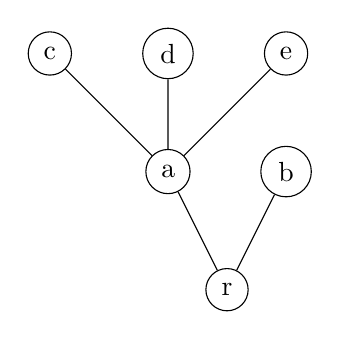
\begin{tikzpicture}[nodes={draw, circle}, -]
\node{r} [grow'=up]
    child { node {a} 
        child { node {c} }
        child { node {d} }
        child { node {e} }
    }
    child { node {b} };
\end{tikzpicture}
\end{center}

The lowermost node~$r$ is the root. Every node other than $r$ has
exactly one parent node immediately below it. We can think of the relation
a node~$x$ stands in to a node~$y$ if $y$ can be reached from $x$ by
following edges upwards as $x$ being an ancestor of~$y$. 

The ancestor relation in a tree is a strict partial order. This
motivates the set-theoretic definition. To state it we need two
concepts. A \emph{minimal element} in a set~$A$ partially ordered
by~$\le$ is !!a{element} $x \in A$ such that for all $y \in A$ we have
that~$x \le y$. A set is \emph{well-ordered} by~$\le$ if every one of
its subsets has a minimal element.

\begin{defn}[Tree]
A \emph{tree} is a pair $T = \tuple{A, \le}$ such that $A$ is a set
and $\le$ is a partial order on~$A$ with a unique minimal element
$r \in A$ (called the \emph{root}) such that for all $x \in A$,
the set $\Setabs{y}{y \le z}$ is well-ordered by~$\le$.
\end{defn}

\begin{defn}[Successors]
Suppose $T = \tuple{A, \le}$ is a tree.
If $x,y \in A$, $x < y$, and there is no $z \in A$ such that
$x < z < y$, then we say that $y$ is a \emph{successor} of~$x$.
\end{defn}

The successors of $x \in A$ are also called its \emph{children}. If
$y$ is a successor of~$x$, then we call $x$ the \emph{predecessor} or
\emph{parent} of~$y$.

\begin{prop}
If $\tuple{A,\le}$ is a tree, then every $x \in A$ other than the root
has at most one predecessor.
\end{prop}

\begin{proof}
  Suppose $y < x$ and $y' < x$ and $y \neq y$. Then both $\{y,
  y'\} \subseteq \Setabs{z}{z<x}$. Since $\Setabs{z}{z<x}$ is
  well-ordered by~$\le$, it has a minimal element, which obviously
  must be either $y$ or~$y'$. So either $y \le y'$ or $y' \le y$. We
  assumed that $y \neq y'$, so actually either $y < y'$ or $y' < y$.
  Since we assumed that $y < x$ and $y' < x$, we furthermore have that
  either $y < y' < x$ or $y' < y < x$. So $y$ and $y'$ cannot both be
  predecessors of~$x$.
\end{proof}

\begin{defn}
A tree $T = \tuple{A, \le}$ is said to be \emph{infinite} if $A$ is an
infinite set, and \emph{finite} otherwise. If $T$ is such that every
$x \in A$ has only finitely many successors, then we say that $T$ is
\emph{finitely branching}.
\end{defn}

\begin{defn}[Branches]
Given a tree $T = \tuple{A, \le}$, a \emph{branch} of~$T$ is a
maximal chain in~$T$, i.e., a set $B \subseteq A$ such that
for any $x, y \in B$ either $x \le y$ or $y \le x$, and for any
$z \in X \setminus B$ there exists $u \in B$ such that neither
$z \le u$ nor $u \le z$.
%
We use $[T]$ to denote the set of all branches of $T$.
\end{defn}

\begin{ex}
A classic example of a finitely branching tree is the
\emph{infinite binary tree} of finite sequences of $0$s and~$1$s,
sometimes denoted $\{0,1\}^*$ or~$\Bin^*$, ordered by the extension
relation $\sqsubseteq$ (e.g., $101 \sqsubseteq 101101$).
Since any binary string can always be extended by adding
a $0$ or a $1$ on the end, this tree contains infinitely
many elements: every element~$s$ has exactly two successors, $s0$ and~$s1$. Its root is the empty sequence $\emptyseq$.
\end{ex}

\begin{ex}
Slightly more generally, the set of finite sequences of natural
numbers~$\Nat^*$ with the extension relation~$\sqsubseteq$ is also a
tree. It is obviously not finitely branching: every $s \in \Nat^*$ has
infinitely many successurs~$sn$, one for every $n \in \Nat$. Every $A
\subseteq \Nat^*$ which is closed under~$\sqsubseteq$ is a
\emph{subtree} of~$\Nat^*$. (That is, $A$ is such that if $s \in A$
and $s' \sqsubseteq s$, then also $s' \in A$.) All finite trees can be
represented as finite subtrees of~$\Nat^*$.
\end{ex}

\begin{prop}[K\H{o}nig's lemma]
If $T = \tuple{A,\le}$ is a finitely branching infinite tree,
then $T$ has an infinite branch.
\end{prop}

A special case of K\H{o}nig's lemma widely used in computability
theory, known as \emph{weak K\H{o}nig's lemma}, is the following: any
infinite subtree of $\{0,1\}^*$ has an infinite branch.

\end{document}
